\documentclass[12pt,a4paper]{article}
\usepackage{ctex}
\usepackage{amsmath,amscd,amsbsy,amssymb,latexsym,url,bm,amsthm}
\usepackage{epsfig,graphicx,subfigure}
\usepackage{enumitem,balance}
\usepackage{wrapfig}
\usepackage{mathrsfs,euscript}
\usepackage[usenames]{xcolor}
\usepackage{hyperref}
\usepackage[vlined,ruled,linesnumbered]{algorithm2e}
\usepackage{array}
\hypersetup{colorlinks=true,linkcolor=black}

\newtheorem{theorem}{Theorem}
\newtheorem{lemma}[theorem]{Lemma}
\newtheorem{proposition}[theorem]{Proposition}
\newtheorem{corollary}[theorem]{Corollary}
\newtheorem{exercise}{Exercise}
\newtheorem*{solution}{Solution}
\newtheorem{definition}{Definition}
\theoremstyle{definition}

\renewcommand{\thefootnote}{\fnsymbol{footnote}}

\newcommand{\postscript}[2]
 {\setlength{\epsfxsize}{#2\hsize}
  \centerline{\epsfbox{#1}}}

\renewcommand{\baselinestretch}{1.0}

\setlength{\oddsidemargin}{-0.365in}
\setlength{\evensidemargin}{-0.365in}
\setlength{\topmargin}{-0.3in}
\setlength{\headheight}{0in}
\setlength{\headsep}{0in}
\setlength{\textheight}{10.1in}
\setlength{\textwidth}{7in}
\makeatletter \renewenvironment{proof}[1][Proof] {\par\pushQED{\qed}\normalfont\topsep6\p@\@plus6\p@\relax\trivlist\item[\hskip\labelsep\bfseries#1\@addpunct{.}]\ignorespaces}{\popQED\endtrivlist\@endpefalse} \makeatother
\makeatletter
\renewenvironment{solution}[1][Solution] {\par\pushQED{\qed}\normalfont\topsep6\p@\@plus6\p@\relax\trivlist\item[\hskip\labelsep\bfseries#1\@addpunct{.}]\ignorespaces}{\popQED\endtrivlist\@endpefalse} \makeatother

\begin{document}
\noindent

%========================================================================
\noindent\framebox[\linewidth]{\shortstack[c]{
\Large{\textbf{Lab07-Amortized Analysis}}\vspace{1mm}\\
CS214-Algorithm and Complexity, Xiaofeng Gao \& Lei Wang, Spring 2021.}}
\begin{center}
\footnotesize{\color{red}$*$ If there is any problem, please contact TA Yihao Xie. }

\footnotesize{\color{blue}$*$ Name:\underline{Xin Xu}  \quad Student ID:\underline{519021910726} \quad Email: \underline{xuxin20010203@sjtu.edu.cn}}
\end{center}
\begin{enumerate}
	\item Suppose we perform a sequence of n operations on a data structure in which the $i$ th 		operation costs $i$ if $i$ is an exact power of 2, and 1 otherwise. Use an accounting method to determine the amortized cost per operation.
	
	\begin{solution}
		The amortized cost per operation is $3$. For any $i$th operation that satisfying $2^k+1\leqslant i\leqslant 2^{k+1},k\geqslant 1$, $1$ is paid for the operation itself for current use, $1$ is paid for the operation itself for future use, the final $1$ is paid for the $j$th operation that $2^{k-1}+1\leqslant j\leqslant 2^k$. So the sum of payment from $2^k+1$ to $2^{k+1}$ is $2^k+2^{k+1}+1$, which is one more that the total actual payment with the same range.
		So, the amortized cost is actually an upper bound of the real cost, and it's the same with the first two operations. In a nutshell, because this amortized analysis provides an upper bound, it's right.
	\end{solution} 

	\item Consider an ordinary \textbf{binary min-heap} data structure with $n$ elements supporting
the instructions \textsc{Insert} and \textsc{Extract-Min} in $O(\log n)$ worst-case time. Give a
potential function $\Phi$ such that the amortized cost of \textsc{Insert} is $O(\log n)$ and the
amortized cost of \textsc{Extract-Min} is $O(1)$, and show that it works.

    \begin{solution}
		Let $D(v_i)$ denotes the height of node $v_i$. The potential function is that $\Phi=\sum_{i = 1}^{n} D(v_i) $. It's easy to know that $\Phi(0)=0, \Phi(n)\geqslant 0$.
		\\ And for the $n$th insertion, if the total height is unchanged, $\Phi(n)-\Phi(n-1)=O(\log n)$, and if the height increases, $\Phi(n)-\Phi(n-1)=O(\log n)$, too. And since the worst case of insertion takes $O(\log n)$, the amortized cost$=O(\log n)$.
		\\ And for the $n$th deletion, $\Phi(n)-\Phi(n-1)=-O(\log n)$ just as discussed above, while the lower down operation takes $O(\log n)$, which can be a compensation. So, the amortized cost is $O(1)$.
	\end{solution}
	
	\item Assume we have a set of arrays $A_0, A_1, A_2,\cdots$, where the $i^{th}$ array $A_i$ has a length of $2^i$. Whenever an element is inserted into the arrays, we always intend to insert it into $A_0$. If $A_0$ is full then we pop the element in $A_0$ off and insert it with the new element into $A_{1}$. (Thus, if $A_{i}$ is already full, we recursively pop all its members off and insert them with the elements popped from $A_0,...,A_{i-1}$ and the new element into $A_{i+1}$ until we find an empty array to store the elements.) An illustrative example is shown in Figure \ref{Fig-MultiArray}. Inserting or popping an element take $O(1)$ time.

	\begin{figure}[!htbp]
	\centering
	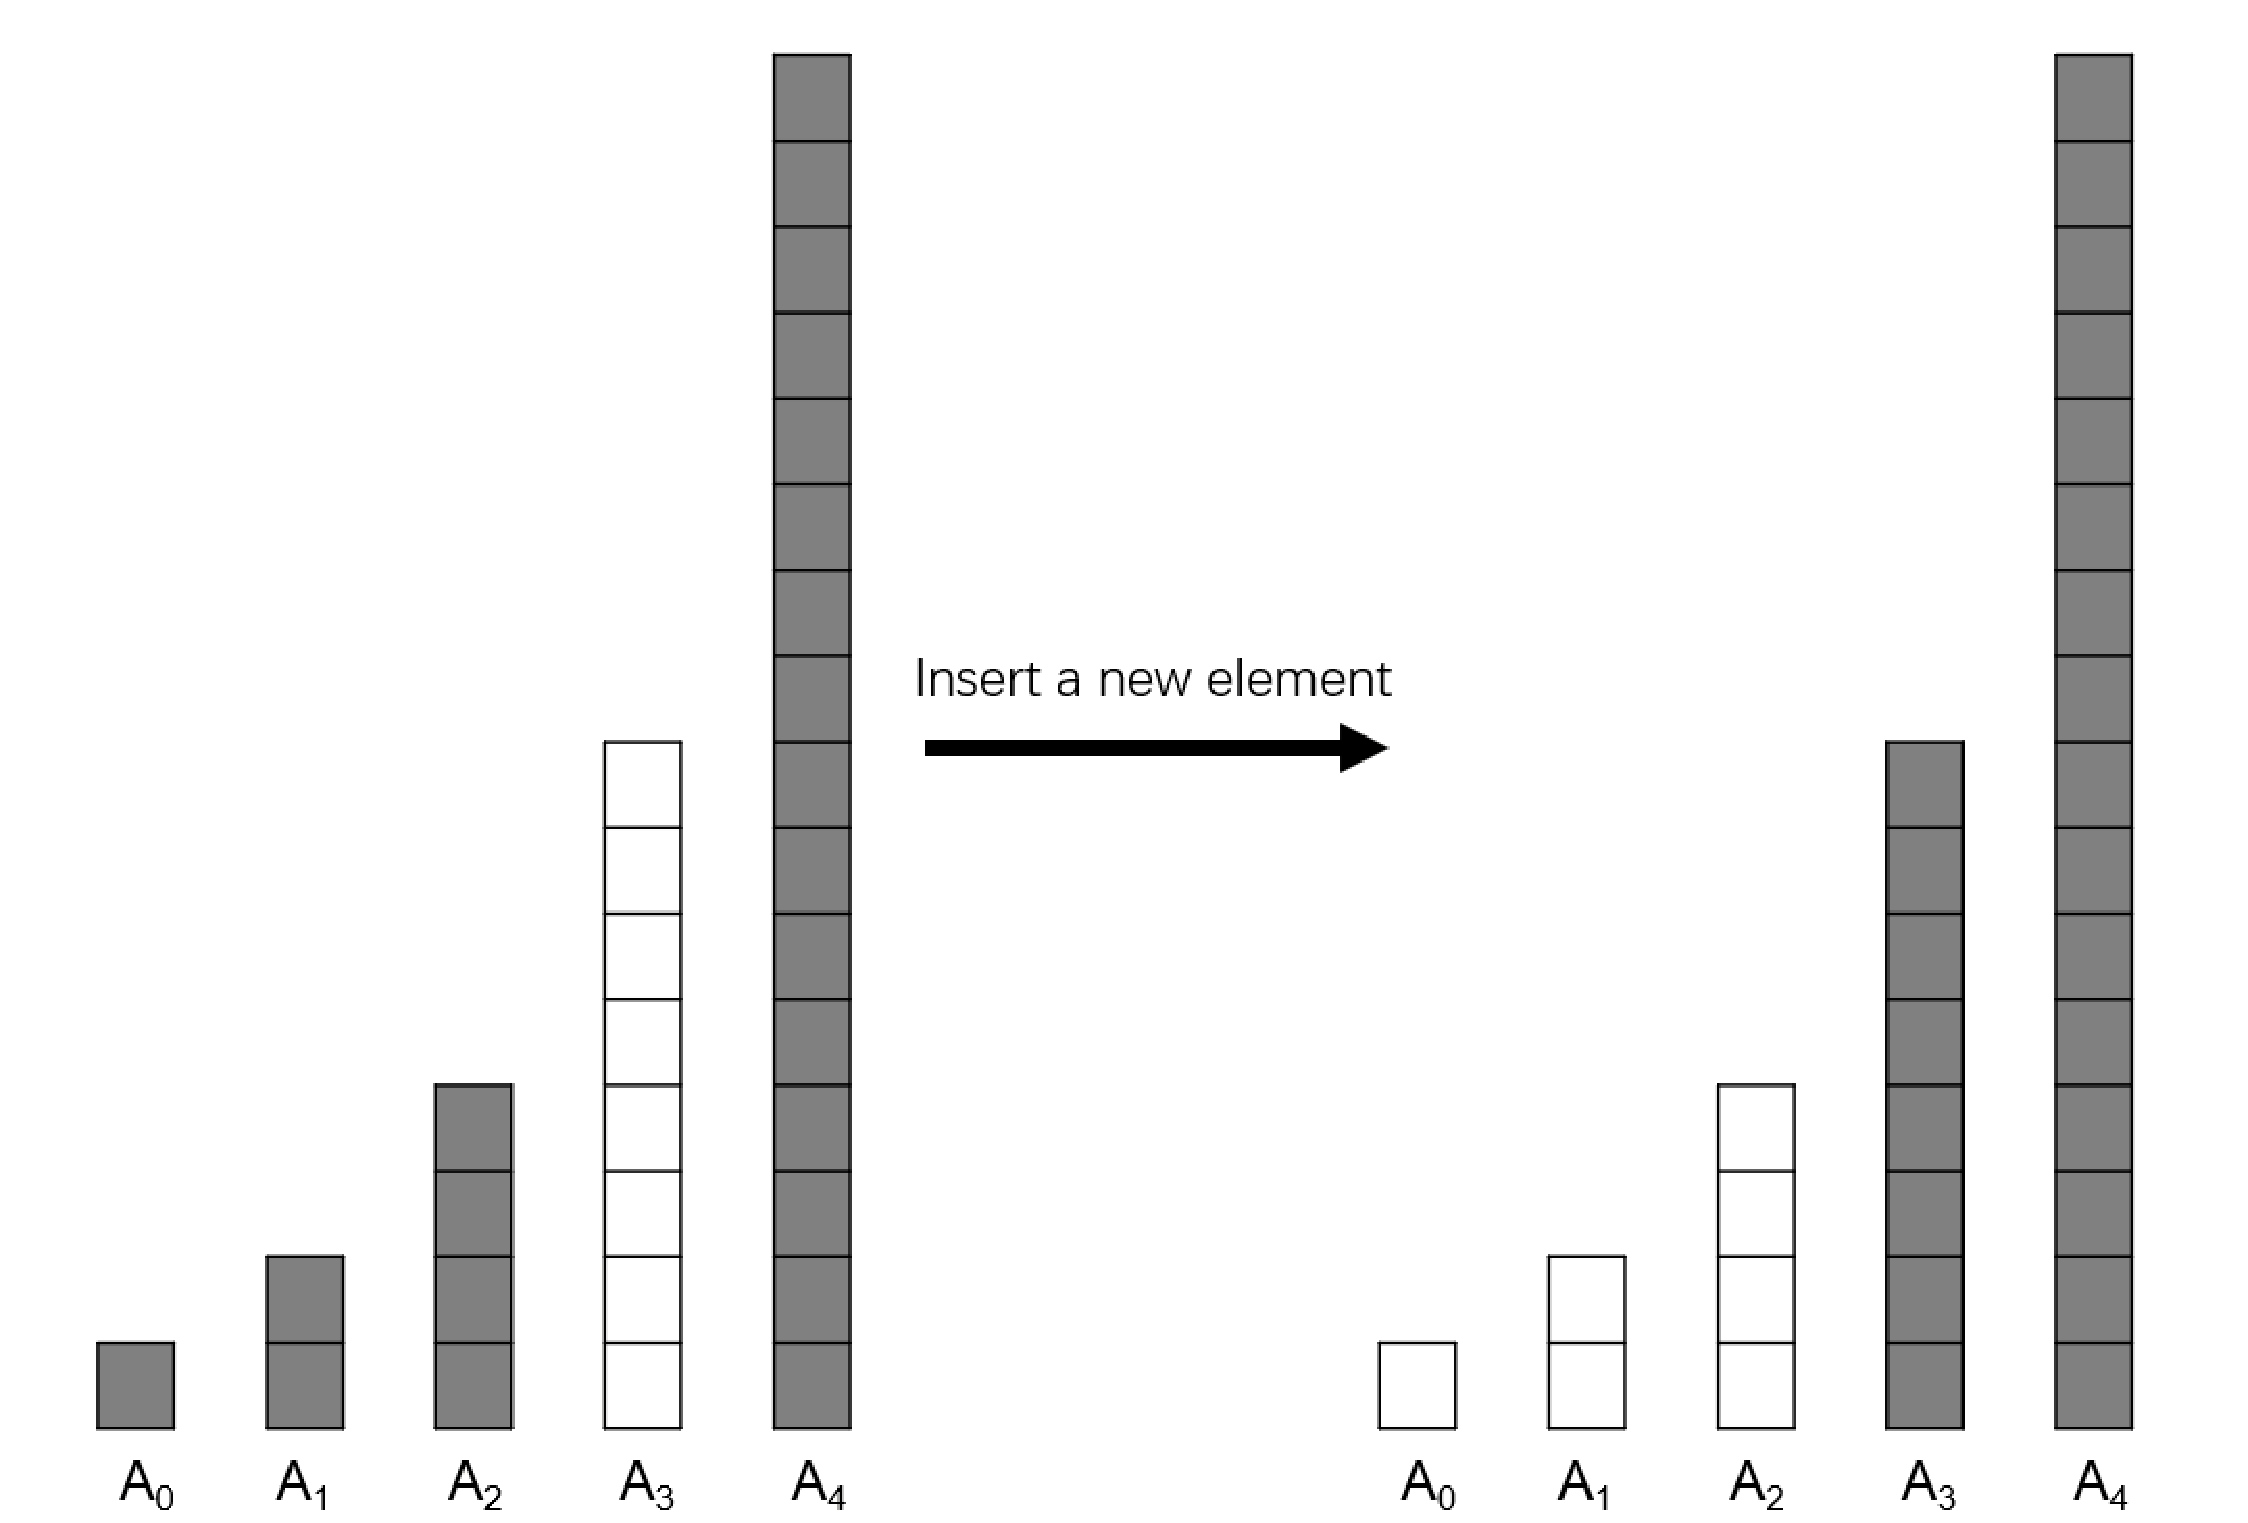
\includegraphics[width=0.5\textwidth]{Fig-MultiArray.pdf}
	\caption{An example of making room for one new element in the set of arrays.}
	\label{Fig-MultiArray}
	\end{figure}

    \begin{enumerate}
        \item In the worst case, how long does it take to add a new element into the set of arrays containing $n$ elements?
        \item Prove that the amortized cost of adding an element is $O(\log n)$ by \emph{Aggregation Analysis}.
        \item If each array $A_i$ is required to be sorted but elements in different arrays have no relationship with each other, how long does it take in the worst case to search an element in the arrays containing $n$ elements? 
\item What is the amortized cost of adding an element in the case of (c) if the comparison between two elements also takes $O(1)$ time?
    \end{enumerate}

	\begin{solution}
		\begin{enumerate}
			\item The worst case is that the first $i$ arrays are all full. If the examination to judge an array full or not takes $O(1)$, the total cost to add a new element into the set of arrays containing $n$ elements is $\log (n+1)+2n+1$. So, in the worst case, it takes $O(n)$.
			\item With the discussion in previous question, the examination to judge an array full or not can be omitted. Thus, the cost list of the first $n$ operations satisfies the follow properties: Firstly, the $2^k,(k\geqslant 1)$th operation costs $2^{k+1}-1$; Secondly, the list is actually a copy and paste process to double itself except the $2^k,(k\geqslant 1)$th operation. 
			\\ So, the total cost of the first $n(n=2^m)$ operations is $n/2+3n/2^2+7n/2^3+15n/2^4+\ldots+2n-1=mn-1+1/n+2n-1=mn+2n+1/n-2$. And the amortized cost is $(mn+2n+1/n-2)/n=O(m)=O(\log n)$.
			\item In the wost case, the search should compare all the elements. So, it takes $O(n)$.
			\item The list of cost has the same structure of problem (b). The $2^k,(k\geqslant 1)$th operation cost includes $2^{k+1}-1$ to locate elements and the cost of comparation. To figure out the cost of comparison, firstly we should know the cost to resort two sorted arrays with the same lengh $n$. In the worst case, the comparison is $2n-1$ for every element in the two arrays must be compared except for the last one.
			So, the comparison cost of $2^k,(k\geqslant 1)$th operation is $\sum_{i = 1}^{k} (2i-1) = k^2<2^{k+1}-1$. So, if we double the value of each element in the list of problem (b), we can get an upper bound of problem (d) as well. And the double process doesn't change the time complexity.
			\\ So, the amortized cost of adding an element in the case (c) considering the cost of comparison is $O(\log n)$ too.
	    \end{enumerate}
	\end{solution} 
	
\end{enumerate}



\textbf{Remark:} Please include your .pdf, .tex files for uploading with standard file names.


%========================================================================
\end{document}
